% ==========================================================================
%  Figure: Explored Nodes by K — Forward vs. Backward
% ==========================================================================
%  Required: \usepackage{pgfplots}  \pgfplotsset{compat=1.18}
% ==========================================================================

\begin{figure}[t]
\centering
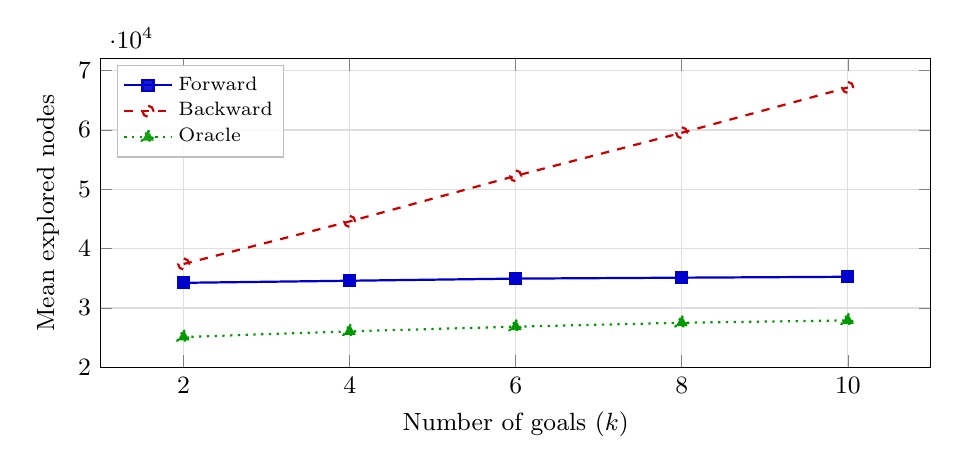
\begin{tikzpicture}
\begin{axis}[
    width=\columnwidth,
    height=5.5cm,
    xlabel={Number of goals ($k$)},
    ylabel={Mean explored nodes},
    xmin=1, xmax=11,
    ymin=20000, ymax=72000,
    xtick={2,4,6,8,10},
    ytick={20000,30000,40000,50000,60000,70000},
    yticklabel style={
        /pgf/number format/fixed,
        /pgf/number format/1000 sep={,},
    },
    grid=major,
    grid style={gray!25},
    tick label style={font=\small},
    label style={font=\small},
    legend style={
        at={(0.02,0.98)},
        anchor=north west,
        font=\scriptsize,
        draw=gray!50,
        fill=white,
        fill opacity=0.9,
        text opacity=1,
        row sep=-1pt,
        inner sep=2pt,
        legend columns=1,
    },
    legend cell align={left},
]

% Forward Search
\addplot[
    color=blue!80!black,
    mark=square*,
    mark size=2pt,
    thick,
    solid,
] coordinates {
    (2,34237.966) (4,34588.588) (6,34946.702)
    (8,35103.476) (10,35256.892)
};
\addlegendentry{Forward}

% Backward Search
\addplot[
    color=red!80!black,
    mark=o,
    mark size=2pt,
    thick,
    dashed,
] coordinates {
    (2,37413.014) (4,44584.454) (6,52264.230)
    (8,59528.692) (10,67160.320)
};
\addlegendentry{Backward}

% Oracle (best of both)
\addplot[
    color=green!60!black,
    mark=triangle*,
    mark size=2.5pt,
    thick,
    dotted,
] coordinates {
    (2,25105.308) (4,26060.614) (6,26848.054)
    (8,27507.168) (10,27899.876)
};
\addlegendentry{Oracle}

\end{axis}
\end{tikzpicture}
\caption{Mean explored nodes as a function of goal count~$k$, averaged
over all problem instances. Forward search remains nearly flat across
$k$-values, while backward search scales linearly with~$k$. The oracle
(per-instance best) shows the potential gain from adaptive direction
selection.}
\label{fig:explored_by_k}
\end{figure}
